%%%%%%%%%%%%%%%%%%%%%%%%%%%%%%%%%%%%%%%%%
% Masters/Doctoral Thesis 
% LaTeX Template
% Version 2.2 (21/11/15)
%
% This template has been downloaded from:
% http://www.LaTeXTemplates.com
%
% Version 2.x major modifications by:
% Vel (vel@latextemplates.com)
%
% This template is based on a template by:
% Steve Gunn/ (http://users.ecs.soton.ac.uk/srg/softwaretools/document/templates/)
% Sunil Patel (http://www.sunilpatel.co.uk/thesis-template/)
%
% Template license:
% CC BY-NC-SA 3.0 (http://creativecommons.org/licenses/by-nc-sa/3.0/)
%
%%%%%%%%%%%%%%%%%%%%%%%%%%%%%%%%%%%%%%%%%

%----------------------------------------------------------------------------------------
%	PACKAGES AND OTHER DOCUMENT CONFIGURATIONS
%----------------------------------------------------------------------------------------

\documentclass[
12pt, % The default document font size, options: 10pt, 11pt, 12pt
% oneside, % Two side (alternating margins) for binding by default, uncomment to switch to one side
english, % ngerman for German
singlespacing, % Single line spacing, alternatives: onehalfspacing or doublespacing
%draft, % Uncomment to enable draft mode (no pictures, no links, overfull hboxes indicated)
%nolistspacing, % If the document is onehalfspacing or doublespacing, uncomment this to set spacing in lists to single
%liststotoc, % Uncomment to add the list of figures/tables/etc to the table of contents
%toctotoc, % Uncomment to add the main table of contents to the table of contents
%parskip, % Uncomment to add space between paragraphs
% nohyperref, % Uncomment to not load the hyperref package
headsepline, % Uncomment to get a line under the header
]{MastersDoctoralThesis} % The class file specifying the document structure

\usepackage[utf8]{inputenc} % Required for inputting international characters
\usepackage[T1]{fontenc} % Output font encoding for international characters

\usepackage{courier} % Use the Palatino font by default
\usepackage{setspace}
\usepackage[backend=biber,style=authoryear,natbib=true]{biblatex} % User the bibtex backend with the authoryear citation style (which resembles APA)

\addbibresource{example.bib} % The filename of the bibliography

\usepackage[autostyle=true]{csquotes} % Required to generate language-dependent quotes in the bibliography
%----------------------------------------------------------------------------------------
%	MARGIN SETTINGS
%----------------------------------------------------------------------------------------

\geometry{
	paper=letterpaper, % Change to letterpaper for US letter
	inner=2.5cm, % Inner margin
	outer=3.8cm, % Outer margin
	bindingoffset=2cm, % Binding offset
	top=1.5cm, % Top margin
	bottom=1.5cm, % Bottom margin
	%showframe,% show how the type block is set on the page
}

%----------------------------------------------------------------------------------------
%	THESIS INFORMATION
%----------------------------------------------------------------------------------------

\thesistitle{A Pipeline for Creation of Genome-Scale Metabolic Reconstructions} % Your thesis title, this is used in the title and abstract, print it elsewhere with \ttitle
\supervisor{Dr. Paul \textsc{Brooks}} % Your supervisor's name, this is used in the title page, print it elsewhere with \supname
\examiner{} % Your examiner's name, this is not currently used anywhere in the template, print it elsewhere with \examname
\degree{Master of Science in Bioinformatics} % Your degree name, this is used in the title page and abstract, print it elsewhere with \degreename
\author{Shaun William \textsc{Norris}} % Your name, this is used in the title page and abstract, print it elsewhere with \authorname
\addresses{} % Your address, this is not currently used anywhere in the template, print it elsewhere with \addressname

\subject{Biological Sciences} % Your subject area, this is not currently used anywhere in the template, print it elsewhere with \subjectname
\keywords{} % Keywords for your thesis, this is not currently used anywhere in the template, print it elsewhere with \keywordnames
\university{\href{http://www.vcu.edu}{Virginia Commonwealth University}} % Your university's name and URL, this is used in the title page and abstract, print it elsewhere with \univname
\department{\href{http://department.university.com}{Bioinformatics}} % Your department's name and URL, this is used in the title page and abstract, print it elsewhere with \deptname
\group{\href{http://researchgroup.university.com}{Paul Brooks Lab}} % Your research group's name and URL, this is used in the title page, print it elsewhere with \groupname
\faculty{\href{http://faculty.university.com}{Dr. Paul Brooks}} % Your faculty's name and URL, this is used in the title page and abstract, print it elsewhere with \facname

\hypersetup{pdftitle=\ttitle} % Set the PDF's title to your title
\hypersetup{pdfauthor=\authorname} % Set the PDF's author to your name
\hypersetup{pdfkeywords=\keywordnames} % Set the PDF's keywords to your keywords

\begin{document}

\frontmatter % Use roman page numbering style (i, ii, iii, iv...) for the pre-content pages

\pagestyle{plain} % Default to the plain heading style until the thesis style is called for the body content

%----------------------------------------------------------------------------------------
%	TITLE PAGE
%----------------------------------------------------------------------------------------

\begin{titlepage}
\begin{center}

\textsc{\LARGE \univname}\\[1.5cm] % University name
\textsc{\Large Master of Science Thesis}\\[0.5cm] % Thesis type

\HRule \\[0.4cm] % Horizontal line
{\huge \bfseries \ttitle}\\[0.4cm] % Thesis title
\HRule \\[1.5cm] % Horizontal line
 
\begin{minipage}{0.4\textwidth}
\begin{flushleft} \large
\emph{Author: Shaun Norris}\\
\href{http://www.newestnorris.com}{\authorname} % Author name - remove the \href bracket to remove the link
\end{flushleft}
\end{minipage}
\begin{minipage}{0.4\textwidth}
\begin{flushright} \large
\emph{Supervisor: Dr. Paul Brooks} \\
\href{https://sites.google.com/a/vcu.edu/jpbrooks/}{\supname} % Supervisor name - remove the \href bracket to remove the link  
\end{flushright}
\end{minipage}\\[3cm]
 
\large \textit{A thesis submitted in fulfillment of the requirements\\ for the degree of \degreename}\\[0.3cm] % University requirement text
\textit{in the}\\[0.4cm]
\groupname\\\deptname\\[2cm] % Research group name and department name
 
{\large \today}\\[4cm] % Date
%\includegraphics{Logo} % University/department logo - uncomment to place it
 
\vfill
\end{center}
\end{titlepage}

%----------------------------------------------------------------------------------------
%	DECLARATION PAGE
%----------------------------------------------------------------------------------------

% \begin{declaration}
% \addchaptertocentry{\authorshipname}
% \doublespacing
% \noindent I, \authorname, declare that this thesis titled, \enquote{\ttitle} and the work presented in it are my own. I confirm that:

% \begin{itemize} 
% \item This work was done wholly or mainly while in candidature for a research degree at this University.
% \item Where any part of this thesis has previously been submitted for a degree or any other qualification at this University or any other institution, this has been clearly stated.
% \item Where I have consulted the published work of others, this is always clearly attributed.
% \item Where I have quoted from the work of others, the source is always given. With the exception of such quotations, this thesis is entirely my own work.
% \item I have acknowledged all main sources of help.
% \item Where the thesis is based on work done by myself jointly with others, I have made clear exactly what was done by others and what I have contributed myself.\\
% \end{itemize}
 
% \noindent Signed:\\
% \rule[0.5em]{25em}{0.5pt} % This prints a line for the signature
 
% \noindent Date:\\
% \rule[0.5em]{25em}{0.5pt} % This prints a line to write the date
% \end{declaration}

% \clearpage

%----------------------------------------------------------------------------------------
%	COPYRIGHT PAGE
%----------------------------------------------------------------------------------------

\vspace*{0.2\textheight}

\begin{center}\noindent{\copyright 2016 Shaun William Norris\\ All Rights Reserved.}\bigbreak \end{center}

%----------------------------------------------------------------------------------------
%	ABSTRACT PAGE
%----------------------------------------------------------------------------------------

\begin{abstract}
\addchaptertocentry{\abstractname} % Add the abstract to the table of contents
\doublespacing
%----- Concise, succinct statement about what was done. -----
%--- Something like: "This work is about developing and using pipelines for metabolic reconstructions" ---
\indent The decreasing costs of next generation sequencing technologies and the increasing speeds at which they work have lead to an abundance of 'omic datasets. The need for tools and methods to analyze, annotate, and model these datasets to better understand biological systems is growing.  Here we present a novel software pipeline to reconstruct the metabolic model of an organism \textit{in silico} starting from its genome sequence and a novel compilation of biological databases to better serve the generation of metabolic models.  We validate these methods using five \textit{Gardnerella vaginalis} strains and compare the gene annotation results to NCBI and the FBA results to Model SEED models.  We found that our gene annotations were larger and highly similar in terms of function and gene types to the gene annotations downloaded from NCBI.  Further, we found that our FBA models required a minimal addition of transport reactions, sources, and escapes indicating that our draft pathway models were very complete. We also found that on average our solutions contained more reactions than the models obtained from Model SEED due to a large amount of baseline reactions and gene products found in ASGARD.
% * <jpbrooks@vcu.edu> 2016-08-31T03:04:47.863Z:
%
% Abstract ends with an incomplete sentence
%
% Abstract ends with an incomplete sentence
%
% ^ <norrissw@vcu.edu> 2016-09-06T19:25:33.214Z.

\end{abstract}

%----------------------------------------------------------------------------------------
%	ACKNOWLEDGEMENTS
%----------------------------------------------------------------------------------------

\begin{acknowledgements}
\addchaptertocentry{\acknowledgementname} % Add the acknowledgements to the table of contents
\doublespacing
\indent\indent The author wishes to thank several people who were pivotal in the completion of this project and his education. First, I would like to thank my advisor and mentor Dr. Paul Brooks whose guidance and oversight were a key element in my journey. Dr. Stephen S. Fong and Dr. Maria C. Rivera for participating on my committee and whose insight and instruction were pivotal in my success. Next, Dr. Allison Johnson and Dr. Herschell Emery whose constant positive encouragement and advice kept me progressing forward. Dr. Jeff Elhai for being my toughest critic and driving me to really think critically about everything I thought I knew.\\
\indent I'd also like to thank Carlisle Childress and the other Center for High Performance Computing staff for all their hard work and helpfulness throughout the years.\\
\indent Last but not least, I would like to thank my family. My wife, AnaClarissa and son Harrison Norris for supporting me throughout this long and challenging journey. My parents James and Katina Norris, my brother Jesse and his wife Alix Norris who have taught me so much and encouraged me to learn more, do more and be a better person. Without all of their love and continued support, I would not have been able to do this.

\end{acknowledgements}

%----------------------------------------------------------------------------------------
%	LIST OF CONTENTS/FIGURES/TABLES PAGES
%----------------------------------------------------------------------------------------
\doublespacing
\tableofcontents % Prints the main table of contents
\doublespacing
\listoffigures % Prints the list of figures
\doublespacing
\listoftables % Prints the list of tables

%----------------------------------------------------------------------------------------
%	ABBREVIATIONS
%----------------------------------------------------------------------------------------

%\begin{abbreviations}{ll} % Include a list of abbreviations (a table of two columns)

%\textbf{LAH} & \textbf{L}ist \textbf{A}bbreviations %\textbf{H}ere\\
%\textbf{WSF} & \textbf{W}hat (it) \textbf{S}tands \textbf{F}or\\

%\end{abbreviations}



%----------------------------------------------------------------------------------------
%	THESIS CONTENT - CHAPTERS
%----------------------------------------------------------------------------------------

\mainmatter % Begin numeric (1,2,3...) page numbering

\pagestyle{thesis} % Return the page headers back to the "thesis" style

% Include the chapters of the thesis as separate files from the Chapters folder
% Uncomment the lines as you write the chapters

% Chapter 1

\chapter{Introduction} % Main chapter title

\label{Chapter1} % For referencing the chapter elsewhere, use \ref{Chapter1} 

%----------------------------------------------------------------------------------------

% Define some commands to keep the formatting separated from the content 
\newcommand{\keyword}[1]{\textbf{#1}}
\newcommand{\tabhead}[1]{\textbf{#1}}
\newcommand{\code}[1]{\texttt{#1}}
\newcommand{\file}[1]{\texttt{\bfseries#1}}
\newcommand{\option}[1]{\texttt{\itshape#1}}
%---- Summary to introduce ---
\indent\indent Historically the hallmark of biology has been the study of the individual molecular components that make up living organisms. However, since the advance of sequencing technology and high performance computing this paradigm has shifted to a more complete approach in which a biologist considers the biological networks that make up the systems that regulate and sustain life for an organism.  Continued research into genomes, gene expression and regulation continues to develop and with it so does our understanding of how each of the elements of an organism interact with one another.  \\
% * <jpbrooks@vcu.edu> 2016-08-31T02:02:42.715Z:
%
% high performance computing biology?
%
% ^ <norrissw@vcu.edu> 2016-09-01T01:45:20.361Z.
\indent Along with this systematic, holistic approach to understanding biological complexity and an increase in computational power have lead to the emergence of new methods for modeling these networks.  By using mathematics one can now represent a metabolic pathway and simulate dynamic and complex biological cellular behaviors. The ability to experimentally obtain genomic data coupled with these modeling approaches has lead to a top-down approach in which the experimental data can be integrated with the models.  This lends greater credibility in the models themselves and the ability to more accurately represent life \textit{in silico}.\\
\indent The ability to represent an organism \textit{in silico} has allowed research to be conducted without the overhead costs associated with a traditional experiment. Using computers you can now predict the outcomes of gene knockouts, and gene up/down regulation. You can also identify drug targets and study complex pathways to identify methods to turn them on, off or bypass them completely.  All of this together has lead to a deepening of our understanding of biology and increased the effectiveness of traditional experiments while reducing costs.\\
\indent However put into the time line of biological research using \textit{in silico} modeling is still very new and was initially cost prohibitive.  It takes a lot of computational overhead to be able to perform these types of experiments.  First, it requires databases that contain experimentally obtained information. Databases hosted by NCBI and other resources are freely available and often can be accessed without downloading the entire dataset. While other databases are proprietary and require you to download them before using them.  Next, the sheer amount of data generated by sequencing, genome annotation, and modeling does require a lot of physical disk space. Most of the intermediate files can be compressed or removed after a functional model is produced but even this can require gigabytes of space per model.  Finally, computational time, as in the actual cost of CPU usage while the modeling procedures are running can also be quite high but due to parallelization and job queuing engines like Sun GridEngine utilizing large amounts of computational time for generating \textit{in silico} has become much easier.\\
% * <jpbrooks@vcu.edu> 2016-08-31T02:04:04.939Z:
%
% > However put
%
% ?
%
% ^ <norrissw@vcu.edu> 2016-09-01T02:14:58.855Z.
\indent The major contributions from our work here is the ability to start from the nucleotide sequence and use our pipeline in a semi-automated fashion to reconstruct the metabolic networks of a given organism.  Previously this process was laborious and there were no tools to parse a genome annotation and derive its reactions based on the gene products determined during the annotation.  Further, we completely redesigned the MetModel into a software tool that will execute all of the necessary steps to create a constraint-based model using flux balance analysis (FBA) all the way to generate the KGML pathway maps from a single execution of the new tool.\\ 
% * <jpbrooks@vcu.edu> 2016-08-31T02:05:56.126Z:
%
% Buy there are tools, like SEED.  Probably cite SEED here and describe its limitations.
%
% Buy there are tools, like SEED.  Probably cite SEED here and describe its limitations.
%
% ^.
%--- A little bit about questions you can ask/answer in silico ---
%--- This is what it requires to do this... databases...storage...computation... etc.
%-------------------------------------------------------------------
%-----------Those Damn Databases-------- Could add details about specific database.
%--- Kegg: Used to be free, no transport reactions, no compartments
%--- SEED: Developed with funding from DOE
%--- Palsson: 
%--- Niti:
\section{Reference Databases}

\indent\indent Most \textit{in silico} tools and projects involve using a reference database at some point. The internet is a great method for sharing information from databases and a number of biological databases already exist to share information about genes, metabolites, and their reaction pathways \citep{keseler_ecocyc:_2013}.\\
\indent However, there is no standardization among these databases and often minimal curation of the data once it has been made available. So not only is there no one source of information that houses all of the data but there is also no standardized form for the information in these databases. This is particularly true when it comes to the metabolic reactions and their metabolites. This makes it difficult to verify the data in these reference databases and it also makes it difficult to obtain a consensus of information from these databases as comparing them is often difficult. \\
\indent Kyoto Encyclopedia of Genes and Genomes (KEGG), is one such database that contains genes, metabolites, reactions, and more for many different organisms\citep{ogata_kegg:_1999}. However, it lacks transport reactions and does not denote where reactions are occurring, i.e. within the cytosol, extracellular or other places.  KEGG is also no longer freely downloadable.  They still have a web page and REST API to access their data, but the user is not informed if they actively update this information or if it lags behind the paid subscribers version. The Model SEED database is another resource for genomes, metabolites, reactions and even full models\citep{overbeek_seed:_2004}. The Model SEED utilizes Rapid Annotation using Subsystems Technology (RAST) which performs the gene annotation and FBA modeling for you. RAST models can utilize genomes uploaded in FASTA or publicly available sequences in the Model SEED database.  The big limitation to using Model SEED is that this data does not appear to be actively curated at this time and thus the possibility of inaccurate or incomplete data exists. When using RAST with Model SEED, another limitation is that during the gap filling step it adds a large number of low-confidence reactions in order to complete pathways. Finally, two manually created databases were created and curated by Dr. Niti Vanee and published by Dr. Bernhard Palsson \citep{vanee_high_2013, shlomi_network-based_2008}. These databases were built to address the missing transport reactions, lack of detail about reaction locations, and otherwise update and curate the missing pieces of data for KEGG and SEED.\\
% * <jpbrooks@vcu.edu> 2016-08-31T02:09:37.236Z:
%
% > perform the modeling for you
%
% This doesn't seem like a drawback.  One of the main limitations of the SEED framework is that it adds too many low-confidence reactions to fill gaps by default.
%
% ^ <norrissw@vcu.edu> 2016-09-01T02:32:00.161Z.
% * <jpbrooks@vcu.edu> 2016-08-31T02:09:02.862Z:
%
% > reated databases
%
% reaction databases
%
% ^ <norrissw@vcu.edu> 2016-09-01T02:23:43.023Z.

%--------CBM----------
\section{Constraint-based Modeling}

\indent\indent Constraint-based modeling is an approach that has been evolving since the 1980s \citep{fell_fat_1986,majewski_simple_1990}. Initially, the approach was first shown to be viable when experimentally obtained metabolic fluxes and growth rates were shown to be consistent with computationally derived fluxes calculated from cellular objective functions \citep{savinell_optimal_1992,schuster_elementary_1994}.  Then in the early 2000s when the ability to sequence whole genomes became more readily accomplished it became possible to link the genome directly to a constraint-based model. This link paved the way for using these models to predict experimental outcomes. For example, gene knockouts and changes in cellular behavior. As biology entered into the age of 'omic data it became possible to incorporate experimentally obtained transcriptomic, exomic, proteomic, and even metabolomic data into these models to further the ability to analyze and experiment \textit{in silico}.\\
% * <jpbrooks@vcu.edu> 2016-08-31T02:11:49.956Z:
%
% > 'omic
%
% Write 'omic instead of 'omic'
%
% ^ <norrissw@vcu.edu> 2016-09-01T02:17:23.892Z.
\indent In general, constraint-based modeling works under the law of conservation of mass and that biomass growth and energy use can be used to predict metabolic fluxes for an organism \citep{schilling_theory_2000,schuster_elementary_1994}. This is accomplished by first curating all the metabolites and reactions determined, or predicted, to be present in an organism. In the case of genome-scale metabolic networks, this is done by creating a stoichiometric matrix. The stoichiometric matrix is a versatile and consistent format present in constraint-based models that indicate the number of molecules used and created in reaction. Here we focus on constraint-based modeling for genome-scale metabolic reconstructions, it has also been used for signaling, transcriptional regulation and macromolecule synthesis \citep{papin_jak-stat_2004,li_identification_2009}.\\
% * <jpbrooks@vcu.edu> 2016-08-31T02:13:08.825Z:
%
% that indicates the number of molecules used and created in each reaction
%
% ^ <norrissw@vcu.edu> 2016-09-01T02:33:26.167Z.
% * <jpbrooks@vcu.edu> 2016-08-31T02:12:34.013Z:
%
% > representing
%
% curating
%
% ^ <norrissw@vcu.edu> 2016-09-01T02:33:29.574Z.
\indent Compared to other modeling methods constraint-based modeling, in general, allows greater influence of metabolic networks for an organism and in a more realistic fashion.  More specifically, an organism \textit{in vivo} is subjected to physical, environmental, and physiochemical inhibitors and thus doesn't have an unlimited growth potential.  By having the ability to apply these constraints makes the \textit{in silico} models more accurate and also expands the ability to perform \textit{in silico} experiments. Utilizing constraint-based modeling we are able to better determine the cellular behaviors of an organism when subjected to different external or internal influences. The end result of this is a series of reaction pathways represented as a flow chart or map that represents what an organism uses to sustain life and these pathways can often vary based on the specific constraints applied to the model. 
% * <jpbrooks@vcu.edu> 2016-08-31T02:14:38.509Z:
%
% >  By considering various constraints allows us to better determine t
%
% reword
%
% ^ <norrissw@vcu.edu> 2016-09-01T02:34:17.508Z.
%------------FBA----------------
\subsection{Flux Balance Analysis}

\indent\indent Flux Balance Analysis (FBA) is one such mathematical approach to modeling and analyzing the networks that make up an organism and is particularly common in genome-scale metabolic network reconstructions \citep{schuster_elementary_1994,varma_stoichiometric_1994,thiele_genome-scale_2009}. FBA is a specific application of linear programming (LP) used to calculate and optimize the flow of metabolites over time through the biochemical reactions present in an organism to determine the steady-state flux distribution that maximizes the biomass yield. Given the stoichiometric matrix (S) and fluxes (v), the steady-state is represented as $Sv = 0$ and defines a system of linear equations. Next, to solve these equations we define an objective function, like biomass, and to predict the maximum growth rate we use $Z =c^Tv$, where c is a vector of zeros with a value of 1 only in the reaction of interest. When we're using the biomass reaction, c has a value of one so we can represent this as:\begin{center} $ Z = v\textsubscript{biomass}$\end{center}
with parameters:
\begin{center} 
$Sv + b^{src} - b^{esc} = 0$

$L \leq v \leq U$

$L^{src} \leq b^{src} \leq U^{src}$

$L^{esc} \leq b^{esc} \leq U^{esc}$
\end{center}
where $L$ and $U$ define the lower and upper bounds for each reaction, and $b^{src}$, $b^{esc}$ are the escape and source reactions specifically\citep{brooks_gap_2012}. Finally we calculate the flux values that maximize $Z$.\\

%-------------------MILP--------------
\subsection{Mixed Integer Linear Programming (MILP)}

\indent\indent Mixed Integer Linear Programming (MILP) is another modeling method.  MILP and LP are both general optimization modeling frameworks and have many applications outside of metabolic reconstructions. In comparing MILP  and LP, MILP is designed to better incorporate and optimize the use of experimentally obtained data into the model as it lets you add integer restrictions variable values\citep{bordbar_constraint-based_2014}. This step helps improve model quality by attempting to reduce false positive and false negative values from experimental data\citep{vanee_high_2013}. A false positive is when a metabolite is predicted to be present but the reaction/gene is associated with producing the metabolite is not actually shown to be present based on experimental evidence. Similarly, a false negative is when a gene or reaction is incorrectly omitted from a model but experimental evidence shows that the associated gene and gene product are in fact present. These false values are believed to be caused by post-transcriptional regulation or alternative flux distributions, which are likely from isozymes and alternative pathways.  In MetModel and Model SEED, MILP is used in FBA-Gap and GapFill which are two different algorithms designed to identify and correct reactions missing from pathways. As mentioned previously MILP can be an effective way to incorporate proteomic and other data into the pathway reconstructions \citep{shlomi_network-based_2008}.\\
% * <jpbrooks@vcu.edu> 2016-08-31T02:16:22.014Z:
%
% >  In short, the MILP algorithm is similar to FBA 
%
% No, delete this sentence.  FBA instances are linear programs (LPs).  My gap-filling models and Shlomi et al's models for reconciling experimental data are examples of MILPs.  LP and MILP are general optimization modeling frameworks.  The only difference is that MILP allows you to add integer restrictions on your variable values.
%
% ^ <norrissw@vcu.edu> 2016-09-01T01:05:48.197Z.
\indent  In the case of MILP we have a problem expressed as: 
% * <jpbrooks@vcu.edu> 2016-08-31T02:19:11.301Z:
%
% > MILP and FBA both calculate fluxes by linear programming. 
%
% No.
%
% ^ <norrissw@vcu.edu> 2016-09-01T01:05:49.821Z.
\begin{center} $maximize \hspace{0.5cm} cx + dy$ \end{center}
with parameters:
\begin{center}
$Ax+By \leq b$

$x \in \mathbb{R}_{+}^n$

$y \in \mathbb{Z}_{+}^p$\end{center}
where $cx + dy$ is the objective function, $Ax+By \leq b$ are constraints, x and y are vectors of the decision variables\citep{brooks_solving_2005}.  We can now determine solutions for our objective function if they exist. It is possible for no solution or multiple solutions to exist, and the solution that provides the best objective function value is called the optimal solution.  When we model using this type of function we look for these optimal solutions if they exist.\\


%------------------FVA----------------

\section{\textit{In Silico} Bacteria Research}

\indent\indent Modeling unicellular organisms \textit{in silico} provides a number of benefits. It allows us to work and analyze with extremophiles and pathogens without expensive equipment or health hazards. It allows us to make predictions about the outcomes for in vivo or in vitro experiments before having to incur the temporal and fiscal costs associated with performing one \citep{langowski_computer_2002}. All of this together allows us to push research of treating and preventing diseases further by focusing and developing our understanding of virulence, pathogenesis and identifying new drug targets\citep{shlomi_network-based_2008}\citep{nurputra_paramyotonia_2012}. In industry different strains or even customized genomes can be tested using these methods and we can select a particular genome or strain of bacteria that provides optimal amounts of a given metabolite which can be collected for purposes like biofuels \citep{nogales_silico_2012}. \\
%-----------ASGARD------------
\subsection{Genome Annotation using ASGARD}

\indent\indent Understanding the genes, their products and the metabolic reactions of \textit{G. vaginalis} is crucial for researching the virulence, transmission, and therapeutics.  We used the genomes of \textit{G. vaginalis} strains obtained from NCBI and other sources, then use the Automated System for Gene Annotation and Metabolic Pathway Reconstruction Using General Sequence Databases (ASGARD) to determine open reading frames and annotate the genome\citep{alves_automated_2007}. \\
\indent ASGARD can take assembled sequences in FASTA file format and perform gene annotation and predicted metabolic pathways. The data provided by ASGARD can be regarded as a draft model, and this creates the first step to a high-quality metabolic model of our organism. \\
\indent ASGARD creates these models by first determining the open reading frames within a genome by comparing it to annotated genomes stored in databases like NCBI Nucleotide and KEGG.  Once the genes and their functions are determined it places them within the appropriate pathways. From here the model can be regarded as a "rough draft" as ASGARD has made an educated guess about the pathways and enzymes present based on translated nucleotide sequence homology only. \\
\indent Using ASGARD thus allows one to take assembled genomic nucleotide sequences in FASTA file format and obtain gene annotation and predicted metabolic pathways. The data provided by ASGARD begins the search for an accurate metabolic model of our organism. We used both well-documented strains (i.e. strains that have already been annotated thoroughly) and novel strains. This "draft" model was then integrated with our MetModel where a series of scripts were used to integrate gene expression data, metabolic data and our other information to increase the accuracy and precision of the draft model.\\

%--------MetModel----------
\subsection{Metabolic Pathway Reconstruction Using MetModel}

\indent\indent For our purposes, ASGARD is just the first step and the model will undergo further revisions as it goes through the MetModel pipeline.  The MetModel pipeline will gap fill pathways then use FBA to derive the reactions rates for optimal growth. It can then be used to build KGML maps of the reaction pathways and if available increase the accuracy and confidence we have in the metabolic reconstruction model by incorporating experimental data. mRNA expression data can be obtained from NCBI Gene Expression Omnibus (GEO) and incorporated during this process in order to provide experimental data to support the analysis and solutions obtained from the FBA. 
% * <jpbrooks@vcu.edu> 2016-08-31T02:23:11.906Z:
%
% > etModel pipeline will use FBA (Flux Balance Analysis) to increase the accuracy and confidence we have in the model.
%
% No.
%
% ^ <jpbrooks@vcu.edu> 2016-08-31T02:24:06.745Z:
%
% Again, what is "the model?"  FBA gives us reaction rates for optimal growth.
%
% ^ <norrissw@vcu.edu> 2016-09-01T11:56:51.079Z.
% * <jpbrooks@vcu.edu> 2016-08-31T02:22:08.577Z:
%
% > the model
%
% It is unclear what you mean by "the model."
%
% ^ <norrissw@vcu.edu> 2016-09-01T11:56:49.617Z.
\indent Finally the model pathways were viewed and reviewed manually using KGML-ED\citep{klukas_dynamic_2007}. \\
\indent MetModel is Python library which can be used in a pipeline to gap-fill reaction pathways determined by ASGARD to then apply a constraint-based modeling approach.  This modeling approach considers all of the potential biochemical reactions and then applies constraints in the same way that an organisms environment, physiochemical, regulatory and evolutionary sources would constrain its growth potential. Thus MetModel allows us to incorporate metabolic data with gene/reaction network, thermodynamics, gene regulation and other information. Using MetModel allows us to consider the states that an organism can and cannot achieve which gives us a broader view as to the factors that are involved in determining an organism's survivability, growth potential and even its ability to produce metabolites under various conditions and with greater accuracy than other modeling tools\citep{roberts_proteomic_2009}. \\
% * <jpbrooks@vcu.edu> 2016-08-31T02:25:26.023Z:
%
% > sing the FBA approach, MetModel
%
% It's not clear what the difference between MetModel and FBA is.
%
% ^ <norrissw@vcu.edu> 2016-09-01T02:39:14.531Z.
% * <jpbrooks@vcu.edu> 2016-08-31T02:24:31.507Z:
%
% >  MetModel is Python library
%
% Maybe cite Seth's T. cruzi paper here.
%
% Maybe cite Seth's T. cruzi paper here.
%
% ^ <norrissw@vcu.edu> 2016-09-01T02:40:40.032Z.
\indent In order for MetModel to perform these tasks it first converts the biochemical reaction network reconstruction into a mathematical form.  To do this we went through three steps, the first is the analysis of the reactions within the network. They usually fall into three main categories like metabolic, regulatory, and signaling. Next, the data derived from this analysis is used to form the stoichiometric matrix. This stoichiometric matrix is the mathematical representation or map where the chemical constraints are applied to the model. Now that we had our mathematical representation of the organism's pathways, flux balance analysis (FBA) can be performed to generate a solution or solutions\citep{orth_what_2010}. FBA calculates the flow of metabolites through the network, and this makes it possible to predict the production rates of metabolites, the growth rate of an organism, and analyze specific pathways and even predict experimental outcomes \citep{lee_complementary_2005}. Put another way these \textit{in silico} models allow predictions of  phenotypes given a set of genes and reactions. For example, we can perform an \textit{in silico} knockout model or we can try to optimize gene products which is particularly useful for nitrogen-fixing bacteria used in biofuel production \citep{nogales_silico_2012}. In the case of pathogens like \textit{G. vaginalis} we can use MetModel to test out new drug designs, or better understand how it might infect and gain a foothold among the normal vaginal bacterial community.\\
\indent Using this modeling approach considers all of the potential biochemical reactions and then applies constraints in the same way that an organism's environment, physiochemical, regulatory and evolutionary sources would constrain its growth potential. Thus MetModel allows us to incorporate metabolic data with gene/reaction network, thermodynamics, gene regulation and other constraints. This approach to modeling allows us to consider the states that an organism can and cannot achieve which gives us a broader view as to the factors that are involved in determining an organism's survivability, growth potential and even its ability to produce metabolites under various conditions.

%----------------------------------------------------------------------------------------Gardnerella--------
\section{Gardnerella}

\indent\indent \textit{Gardnerella} is a genus of bacteria for which \textit{G. vaginalis} is presently the only known species. \textit{G. vaginalis} is a clinically significant bacterium that can disrupt the normal vaginal flora and cause bacterial vaginosis (BV). BV is a major medical problem, causing discomfort to millions of women every year and has been shown to cause complications for many pregnant women resulting in preterm labor and birth which may result in death or long-term health problems for the baby. Many patients with BV are asymptomatic but occasionally have yellow or gray discharge, irritation, or a foul odor. Diagnosing BV can be difficult especially if the patient is asymptomatic. Figure ~\ref{fig:ClueCells} shows a diagrammatic depiction of how these bacterial cells are identified once stained. \textit{G. vaginalis} is not considered to be the single microbe inducing BV but rather a signal that the normal vaginal tract flora has been disrupted, thus paving the way for other anaerobes to work synergistically to reduce the protective, hydrogen peroxide producing {\it Lactobacillus} species that suppress the harmful bacteria from proliferating. Further, the \textit{G. vaginalis} cells are so small they do not reliably show up as gram-positive and thus can be difficult to detect. Presently, the main treatment for patients with BV caused by \textit{G. vaginalis} are antibiotics such as clindamycin or metronidazole.\\
\begin{figure}[h]
\centering
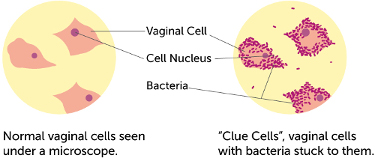
\includegraphics{Figures/ClueCells}
\decoRule
\caption[Clue Cells]{Artist's rendering of how a clinician is able to use microscopy to identify \textit{G. vaginalis} cells that have infected vaginal tissue. Image reprinted with permission from: \citep{_bacterial_????} }
\label{fig:ClueCells}
\end{figure}
\indent\textit{Gardnerella vaginalis} is a gram-variable anaerobic coccobacilli. It is a facultative anaerobe and can metabolize glucose under both aerobic and anaerobic conditions, and has a complex metabolism \citep{patterson_analysis_2010}. It is the sole member of the \textit{Gardnerella} genus and is a small (\(1.0  \mu m\)), non-motile and nonspore-forming bacterium. The \textit{G. vaginalis} genome is a circular DNA and is without plasmids. Within \textit{G. vaginalis} there are genetic variants that include both virulent and avirulent strains. It is considered to be a key component in the initiation and progression of BV \citep{schwebke_role_2014}. Models of the pathogenesis of BV suggest the virulent stains of \textit{G. vaginalis} are usually transmitted through sexual intercourse and its virulence factors allow it to adhere to vaginal epithelial tissue.  Once attached to epithelial cells it creates a biofilm where a community of normally dormant vaginal anaerobes flourish. \textit{Gardnerella vaginalis} also exhibits cytotoxic activities \citep{patterson_analysis_2010}. Once established this biofilm community then aggressively competes with microorganisms of the typical vaginal flora. For example, the predominant \textit{Lactobacillus} populations that help regulate a healthy pH, and creates conditions for an overgrowth of \textit{G. vaginalis} and its associated pathogenic anaerobes. This microfloral replacement results in the clinical symptoms associated with BV (odor, discomfort, itch etc.). Studying the pathogens' genes gives biochemical and metabolic information to interpret its cooperative and competitive interactions with its human host and co-occurring species, suggesting how it overgrows and out-competes the established healthy microflora. Understanding the etiology of the disease will hopefully give insights into the best methods to prevent and control it.   \\
\indent There are over 1,365 genes in the reference genome of \textit{Gardnerella vaginalis ATCC 14019}. Not all of the \textit{G. vaginalis} strains identified are virulent and more research is needed in order to understand the virulence factors. It does appear that \textit{G. vaginalis} forms symbiotic relationships with other vaginal anaerobes that are normally dormant, and these relationships contribute to its success, resulting in symptoms and progression of BV\citep{gardner_pathogenicity_1983,schwebke_role_2014}.
% Chapter 2

\chapter{Curating a Database for Metabolic Reconstructions} % Main chapter title

\label{Chapter2} % For referencing the chapter elsewhere, use \ref{Chapter2} 

%----------------------------------------------------------------------------------------Those Damn Databases Again----------
\section{Reference Databases}

\indent\indent Upon starting this project MetModel already used a comma separated file (CSV) that contained reactions from the Kyoto Encyclopedia of Genes and Genomes (KEGG), the SEED database and contributions from Dr. Niti Vanee and published by Dr. Bernhard Palsson \citep{ogata_kegg:_1999, overbeek_seed:_2004, vanee_genome_2009, shlomi_network-based_2008}. However, despite these reactions all being in a single file, there was no way to relate the reactions to each other.  It was apparent that there were duplicate reactions that were represented in different formats and that the overall process of looking up reactions could be improved by creating a standardized format for the reactions. \clearpage

\subsection{Reference Database Collection and Clean Up}

\indent\indent To collect and clean up the information housed in the Kyoto Encyclopedia of Genes and Genomes (KEGG), Chemical Entities of Biological Interest (ChEBI), and the SEED database, when SQL or CSV files were available they were downloaded, but often information needed to be scraped from these online sources\citep{ogata_kegg:_1999, degtyarenko_chebi:_2008, overbeek_seed:_2004}. Web scraping was performed using Scrapy \citep{_scrapy_????}. Scrapy is a web scraping toolkit written in Python. Scrapy made it possible to download all of the information from these websites and simultaneously format it in a standardized way that we could then parse and load into a PostgreSQL database.\\
\begin{table}
\caption{An example of the data stored in new Compound Reference SQL Table.}
\label{tab:CPDID}
\centering
\begin{tabular}{l l l l l l}
\toprule
\tabhead{KEGG ID} & 
\tabhead{SEED ID} & \tabhead{CHEBI ID}&
\tabhead{VANEE} &
\tabhead{PALSSON} &
\tabhead{Name} \\
\midrule
C00001 & cpd00001 & 15377 & H$_2$O & H$_2$O & Water\\
C00002 & cpd00002 & 15422 & ATP & ATP & ATP \\
C00003 & cpd00003 & 13389 & NAD+ & NAD+ & NAD \\
C00004 & cpd00004 & 16908 & NADH & NADH & NADH \\
\bottomrule\\
\end{tabular}
\end{table}
\indent Loading all of this data into a SQL database made it possible to query this data simultaneously. Having all this data in a single place then allowed us to develop a Python pipeline to query each of these sources concurrently to return the identifiers for a given compound or reaction associated within each of these respective databases. This allowed for the creation of a standardized format and thus reduce duplicate information. For example, one of the biggest issues with the reactions is how the compounds are named. KEGG may refer to water as H$_2$O while SEED may actually refer to it as water. In another example, when water is donating a proton in a particular reaction some databases referred this as just H while in others H+,H$_2$O or even H$_3$O$^+$ even though the reaction was the same and clearly involved a single H (proton) being donated. With the methods described here we obtained the full set of metabolites and their associated information and we used pattern matching to automate the translation of these reactions into a standardized format using the KEGG identifiers (if available) for that given compound. The format took after the form of the KEGG identifiers like $C00001 + C00404 <=> C02174$ where C00001 represents H2O, C00404 represents polyphosphate and C02174 represents oligophosphate. If the compound was not found in the KEGG database but was present in others it was assigned a UNK000X identifier. Table \ref{tab:CPDID} shows a sample of the results from the compound reference table. \\
\indent Any reactions not automatically translated were flagged and reviewed manually.  Once all of the compounds and reactions were in the same format we then quickly created a mapping of like equations.  This mapping was stored in a PostgreSQL table so that we could quickly access relevant information in each database by retrieving its appropriate ID from the database. Table \ref{tab:RXNID} shows a sample of the results from the reaction reference table. \\
\indent Once completed, using Python and SQL statements, a quick and easy method to retrieve all of the relevant data and analysis resources from these pathway/genome databases was created. This rapid look-up helped us obtain and verify metabolic pathways and enzymes derived from experimental results published in the scientific literature. In particular, this is needed because unfortunately these databases are not always well maintained and information in any one source may be out of date or inaccurate. By using this method we kept up to date in order to best assign and verify the function for the majority of genes in selected genomes.

\begin{table}
\caption{An example of the data stored in new Reaction Reference SQL Table.}
\label{tab:RXNID}
\centering
\begin{tabular}{l l l l l l}
\toprule
\tabhead{KEGG ID} & 
\tabhead{SEED ID} &
\tabhead{NITI} &
\tabhead{PALSSON} &
\tabhead{EC Number(s)} \\
\midrule
R01867 & rxn09563 & R\_DHORD4 & R\_DHORD4 & 1.3.3.1 \\
R04749 & rxn03250 & R\_ECOAH2 & R\_ECOAH2 & 4.2.1.17|4.2.1.74  \\
R00405 & rxn00285 & R\_SUCOAS & R\_SUCOAS &  6.2.1.4|6.2.1.5 \\
R03146 & rxn10115 & R\_FDH3 & R\_FDH3 &  1.2.2.1\\
\bottomrule\\
\end{tabular}
\end{table}
%----------------------------------------------------------------------------------------
 
% Chapter 3

\chapter{From Sequence to Metabolic Reconstruction} % Main chapter title

\label{Chapter3} % For referencing the chapter elsewhere, use \ref{Chapter3}

%---------------------------------------------------------------------------------------- This is the pipeline
%---- Overview of algorithm process ---
\indent\indent ASGARD and MetModel are tools that perform genome annotation, and metabolic pathway reconstruction respectively. Both tools do their job well but it is not easy or intuitive to use them and especially not together.  For starters, neither of these tools provide adequate documentation on how to use them or the specific file formats and data that they require to run.  Next, they don't integrate well on their own so it was not possible to start from the raw nucleotide sequence data and build a metabolic model from there before our work. Now while the process is still not completely automated, that decision was actually intentional as it is helpful to be able to review the output from each step in the workflow in order to ensure nothing is missing and manually add or remove reactions or metabolites if need be.  Figure 3-1 shows an overview of the pipeline and the steps that MetModel uses to perform FBA and generate the KGML reaction maps.  Our specific contributions are highlighted in yellow, and the scoring function which was developed by Stephen Wunsch and then incorporated into the pipeline is highlighted in green\citep{wunsch_stephen_a._scoring_2016}.\\
% * <jpbrooks@vcu.edu> 2016-08-31T02:35:17.916Z:
%
% > respective jobs
%
% describe the jobs
% ADD Wunsch citation here
% ^ <norrissw@vcu.edu> 2016-09-01T02:47:10.477Z.
\begin{figure}[h]
\centering
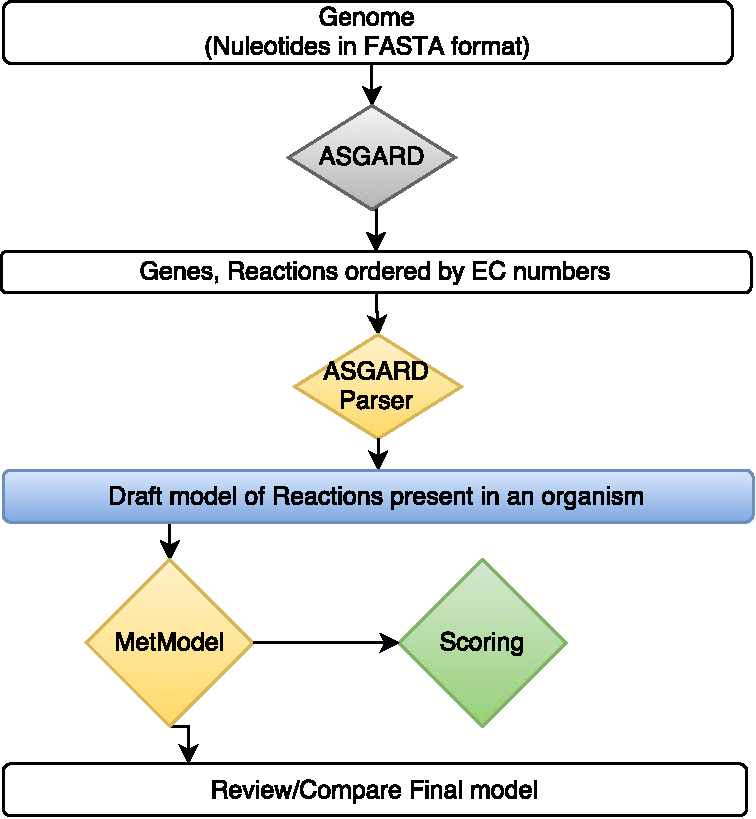
\includegraphics{Figures/Pipeline}
\decoRule
\caption[Pipeline Workflow]{This shows the workflow used to reconstruct a metabolic network starting from just the nucleotide sequence of an organism's genome. My specific contributions are highlighted in yellow, and the collaborative effort on the scoring mechanism is highlighted in Green.}
\label{fig:Pipeline}
\end{figure}

%---- The two main contributions are: ---
\section{ASGARD Parser}

\indent As mentioned before, ASGARD is a tool for determining open reading frames and then annotating genes, then uses this protein product information to determine the reactions present in the gene.  It works by supplying a FASTA formatted file, and the output is a BED file which contains the enzyme commission numbers (EC) that were predicted to be present in the organism.  This is a big step toward building a complete pathway model, but there were still missing steps before a model could be generated.  First, a python script was developed and used to parse the EC numbers from the output, and searched within the new reference database for the associated reactions, pathways, and if possible genes/gene products associated with them.  This information was then used to build the list of reactions needed to run MetModel.\\

%----- 1. Call ASGARD, get EC Numbers, Build 'Model' for MetModel, Call MetModel Pipeline through met_model script------
%-------- A Table showing pathway/reaction counts would be good here %----------
\section{MetModel Pipeline}

\indent\indent Once the data from ASGARD was formatted properly it could now be used with the MetModel pipeline.  In order to use MetModel originally you either had to create your own scripts and call the appropriate functions or for convenience four separate static scripts were written as example usages and each had to be tailored specifically to the model that was being run and each script performed a single step which needed to be executed independently and in order. As a part of this work all of the function calls, data, and information that was contained in these four separate scripts were incorporated into one Python script which created an user friendly, reusable software tool. The new script uses command line arguments to run different procedures and can be run dynamically without having to alter the code of the scripts themselves.  Doing this created a semi-automated process in which a user can use to pause at each step if he or she wishes to manually intervene or review the files produced before completing the entirety of the MetModel FBA process. \\ 
% * <jpbrooks@vcu.edu> 2016-08-31T02:37:16.572Z:
%
% > MetModel was originally used in four separate static scripts that all had to be run independently.
%
% No, MetModel is a collection of Python functions.  There were four convenience scripts created to call these functions.
%
% ^ <norrissw@vcu.edu> 2016-09-01T02:49:08.418Z.
\indent This tool we created allows the user to also select which steps in the pathway to perform, the default being all four.  Step 1 the MetModel pipeline adds transport reactions and if desired you can even attempt to build a model from this information. In step 2 we perform gap filling to complete the pathways and use FBA to determine the reaction rates and fluxes. In step 3, if experimental data is available it can be incorporated. In Step 4, the KGML maps are rendered.	These models were then scored and validated using the scoring function implemented by Stephen Wunsch\citep{wunsch_stephen_a._scoring_2016}.  \\
% * <jpbrooks@vcu.edu> 2016-08-31T02:39:24.708Z:
% again add WUNSCH citation
% > the final FBA is performed
%
% It's the same FBA instance, so really Step 4 is only to generate KGML maps.
%
% ^ <norrissw@vcu.edu> 2016-09-01T02:50:04.172Z.
% * <jpbrooks@vcu.edu> 2016-08-31T02:38:46.862Z:
%
% > FBA to generate a model.
%
% FBA does not generate a model.  It provides reaction rates/fluxes.
%
% ^ <norrissw@vcu.edu> 2016-09-01T02:50:05.159Z.

\indent The scoring method is designed to give a relative confidence score in the pathways that were included in the final model. It is the result of a collaborative effor between Dr. Stephen Fong, Stephen Wunsch and myself and was ultimately implemented by Stephen Wunsch, a PSM Bioinformatics graduate student\citep{wunsch_stephen_a._scoring_2016}
% ---It is the result of a collaboratative effort between Dr. Stephen Fong, myself and Stephen Wunsch. -- I don't know how to say this?
The method he developed works by using BeautifulSoup, a Python library and framework for webscraping, similar to Scrapy. It takes an individual reaction within a network and uses BeautifulSoup to seek out publications that provide experimental evidence of that reaction within the pathway and organism.  The more unique data it can discover the higher the score.  It then outputs these scores on a scale of 1-10, 1 being the lowest and 10 being the highest. A score of 10 indicates that the gene, protein, and reaction all have at least one primary journal article supporting them that contains experimental evidence that explicitly shows that the gene products and reactions are present in the organism. The score decreases from there when evidence cannot be found for example, a score of 5 indicates that the gene-protein reaction (GPR) have been associated with multiple EC numbers but are without publications that provide direct experimental evidence to support them.\\
% Chapter 4

\chapter{Comparison of Metabolism using Five \textit{G. Vaginalis} Strains} % Main chapter title

\label{Chapter4} % For referencing the chapter elsewhere, use \ref{Chapter4}

%----------------------------------------------------------------------------------------
%---- A table showing the reaction scores from each model show go here. ----
%------ Sequences ---------
\section{\textit{Gardnerella vaginalis} Nucleotide Sequences}
\indent\indent The nucleotide sequences of the genomes from five different \textit{Gardnerella vaginalis} strains: 5-1, 41V, 101, AMD, and ATCC 14019, were obtained from NCBI Nucleotide database. These nucleotide sequences in FASTA format were then uploaded to our computing cluster where they could be annotated and then reconstructed into models. Initial ASGARD annotations were also provided in Excel format containing ASGARD output from these five strains and others.  This data was used for comparison against our ASGARD runs. We also downloaded the metabolic models generated using Model SEED for these same strains so that our results could be compared.\\
% * <jpbrooks@vcu.edu> 2016-08-31T02:41:53.839Z:
%
% What about the annotations that Myrna provided?
%
% ^ <norrissw@vcu.edu> 2016-09-01T02:52:07.509Z.

%-----------ASGARD------------
\section{Genome Annotation using ASGARD}
\begin{table}
\caption{Comparison of Gene Annotations from ASGARD, NCBI and Model SEED.}
\label{tab:gene_numbers}
\centering
\begin{tabular}{l l l l}
\toprule
\tabhead{\textit{G. vaginalis} Strain} & \tabhead{ASGARD} & \tabhead{NCBI} & \tabhead{Model SEED}\\
\midrule
5-1 & 2140 & 1271 & 345 \\
AMD & 2417 & 1190 & 339 \\
101 & 1833 & 1150 & 329 \\
ATCC 14019 & 1485 & 1366 & 380 \\
41V & 1210 & 1230 & 371 \\
\bottomrule\\
\end{tabular}
\end{table}
\indent\indent Understanding the genes, their products and the metabolic reactions of \textit{G. vaginalis} is crucial for researching the virulence, transmission, and therapeutics.  We used genomes of \textit{G. vaginalis} strains obtained from NCBI and other sources, then used the Automated System for Gene Annotation and Metabolic Pathway Reconstruction Using General Sequence Databases (ASGARD) to determine open reading frames and annotate the genome\citep{alves_automated_2007}. \\

\indent By using ASGARD we were able to take the assembled nucleotide sequences, obtained from NCBI's nucleotide database, in FASTA file format and obtain gene annotation and predicted metabolic pathways. The data provided by ASGARD is a set of reactions for a given pathway, determined by the genes which were present during the annotation. We regarded this data as a draft model for the reactions present in each of the \textit{Gardnerella} strains. Each of these draft models was then run through our ASGARD parser script, which extracted the EC numbers in each of the pathways that were determined by ASGARD to be present.  The EC numbers were then used to obtained the specific reactions and when possible associated genes, by querying our reference database. This information was then put into the appropriate text format so that it could move on to the next step of being put through the MetModel pipeline where we would integrate gene expression data, metabolic data and our other information to increase the accuracy of the model. \\
% * <jpbrooks@vcu.edu> 2016-08-31T02:46:24.266Z:
%
% > increase the accuracy and precision of the model. 
%
% If a model is a collection of reactions, how does MetModel "increase the precision?"
%
% ^ <norrissw@vcu.edu> 2016-09-01T02:53:44.480Z.
% * <jpbrooks@vcu.edu> 2016-08-31T02:45:30.644Z:
%
% >  draft models 
%
% So is a model a collection of reactions?
%
% ^ <norrissw@vcu.edu> 2016-09-01T02:53:45.624Z.

\indent To validate the gene annotation performed by ASGARD we compared the Gene Feature Format (GFF) file created by ASGARD and the GFF files obtained from NCBI and the Model SEED table containing genes and their reactions. The GFF files contain genes and their coordinates and we compared them both by looking at the number of genes and the name of the gene. We removed redundant genes within the ASGARD GFF and NCBI GFF files before performing this comparison. Table \ref{tab:gene_numbers} shows the results of this comparison. Overall, ASGARD showed an average of 72\% similarity in the genes determined to be present between the strains when compared to the genes present in the NCBI annotations for each strain. Although, there were was a strong deviation for the AMD strain which was only 49\% similar and ASGARD determined a significantly higher amount of genes found compared to the number present in the reference strain. On the contrary, the 41V strain was 98\% similar. In all cases, ASGARD determined a larger number of genes when compared to the number of genes predicted by Model SEED. This difference appeared to be due to Model SEED only regarding genes in the PATRIC database that have EC numbers attached to them \citep{devoid_automated_2013}. \\
\indent It is clear that the ASGARD algorithm is also more greedy than the Model SEED algorithm when it comes to gene and reaction pathway determination. However, since these strains lacked experimental evidence for transcriptomic or proteomic data it is unknown if the accuracy of ASGARD to determine open reading frames and predict the genes present in an organism is better or worse than Model SEED's annotation process.  This increased amount of genes, and therefore pathways, as predicted initially by ASGARD and used as a starting point my MetModel, did eliminate the need for gapfilling during pathway reconstruction, which is a positive outcome and could indicate the ASGARD is more thorough and accurate when annotating a genome. \clearpage

%--------MetModel----------
\section{Metabolic Pathway Reconstruction Using MetModel}

\indent\indent Each of the genes and reaction sets for all of the strains of \textit{Gardnerella} obtained from ASGARD, and parsed out into the appropriate format expected by MetModel were then run through the MetModel pipeline using the new MetModel tool. Our MetModel tool allows a user to start from a file that contains gene-reaction products and run through four different steps to take a set of reactions and reconstruct the individual reaction pathways in order to model an organism. For all of the strains of \textit{Gardnerella} we ran all through the steps of the MetModel script, excluding step 3 as no experimental proteomic data was available for any of the individual strains. The MetModel pipeline then allowed us to use the set of genes and reaction pathways determined by ASGARD to then apply the FBA constraint-based modeling approach.  \\
% * <jpbrooks@vcu.edu> 2016-08-31T02:48:24.970Z:
%
% >  run through four different steps to build a model
%
% Again, "build a model" is ambiguous and not defined.
%
% ^ <jpbrooks@vcu.edu> 2016-08-31T02:50:02.059Z:
%
% I don't see how writing KEGG maps is building a model.
%
% ^ <norrissw@vcu.edu> 2016-09-01T02:54:41.126Z.

\indent The reconstructions created by MetModel were then compared to models available in the Model SEED database. We found that on average our reconstructions had 474 more reactions than the Model SEED reconstructions.  Another major difference to note is that during the gap-filling step in the MetModel pipeline no reactions needed to be added in order to complete pathways. Of course as previously mentioned we did add transports and escapes during the first iteration in the MetModel pipeline. It appears that MetModel ended up with more reactions because the reaction data parsed ASGARD had a much higher number of genes and reactions. While some of these reactions were removed by MetModel a significant amount stayed and thus increased the number of reactions compared to Model SEED. Comparing MetModel reconstructions to the Model SEED reconstructions it at first seemed odd there was a difference of over 400 reactions, but when looking at other models, for example, \textit{Escherichia coli K-12 MG1655} it contains 1366 genes and 2251 reactions in MetModel reconstruction and in the Orth et al. 2011 published model while in Model SEED it contains only 1132 genes and 1632 reactions. Further, the \textit{E. coli} only had transports and escapes added prior to the gap-filling step (GapFill) in MetModel while in Model SEED 38 reactions were added\citep{brooks_gap_2012}.\\
\indent One of the principle reasons for the differences in the number of genes present from each of the annotation sources is the algorithms used to determine the genes present. ASGARD uses a greedy algorithm and it appears it could be overestimating the number of genes present.  NCBI, on the other hand, uses information uploaded by its users so depending on the methods used to annotate the organism's genome the accuracy can vary.  Further, the NCBI data is not always well curated so it is also possible that some older methods and technologies were used to sequence and annotate these organisms which could again affect the accuracy of the sequences and accuracy of the gene annotations.  Finally, Model Seed appears to be only including genes that are present in the PATRIC database and have known enzymes catalog identifiers attached to them.  While this approach does ensure the genes predicted to be present have a high degree of experimental and literature support it is likely missing out on a lot of genes whose functions have limited evidence available but are, in fact, present in the organism.
% * <jpbrooks@vcu.edu> 2016-08-31T02:55:39.388Z:
%
% > our MetModel 
%
% What is "our MetModel?"
%
% ^ <norrissw@vcu.edu> 2016-09-01T02:55:33.525Z.
% * <jpbrooks@vcu.edu> 2016-08-31T02:54:21.955Z:
%
% > during prior
%
% ?
%
% ^ <norrissw@vcu.edu> 2016-09-01T02:55:34.605Z.
% * <jpbrooks@vcu.edu> 2016-08-31T02:53:00.332Z:
%
% > gapfill
%
% It should be GapFill and needs a citation.  GapFill adds reactions until every metabolite can be produced.  Our gap-filling algorithm (FBA-GAP) only adds reactions that are needed to produce biomass, so it should be much fewer.
%
% ^ <norrissw@vcu.edu> 2016-09-01T03:03:02.342Z.
% * <jpbrooks@vcu.edu> 2016-08-31T02:52:34.785Z:
%
% > during prior t
%
% which one?
%
% ^ <norrissw@vcu.edu> 2016-09-01T03:03:01.143Z.
% * <jpbrooks@vcu.edu> 2016-08-31T02:51:18.045Z:
%
% > n our MetModel pipeline no reactions needed to be added in order to complete pathways. 
%
% So how did we end up with more reactions then?
%
% ^ <norrissw@vcu.edu> 2016-09-01T03:02:58.535Z.
% * <jpbrooks@vcu.edu> 2016-08-31T02:50:40.189Z:
%
% > 474 more reactions than the Model SEED
%
% I would have expected fewer.  What are these additional reactions?
%
% ^.
\begin{table}
\caption{Comparing the number and types of Reactions in MetModel vs Model SEED.}
\label{tab:numrxn}
\centering
\begin{tabular}{l l l}
\toprule
\tabhead{\textit{G. vaginalis} Strain} & \tabhead{MetModel total} &  \tabhead{Model SEED total}  \\
\midrule
5-1 & 1217 & 761 \\
AMD & 1248 & 744 \\
101 & 1220 & 760 \\
ATCC 14019 & 1232 & 769 \\
41V & 1235 & 745 \\
\bottomrule\\
\end{tabular}
\end{table}
%---- Scoring of Models, do I need this? -----
\section{MetModel Validation and Scoring}

\begin{table}
\caption{The Average Confidence scores of the five strains.}
\label{tab:strain_scores}
\centering
\begin{tabular}{l l l}
\toprule
\tabhead{\textit{G. vaginalis} Strain} & \tabhead{Score} \\
\midrule
5-1 & 1.92\\
AMD & 1.84\\
101 & 1.97 \\
ATCC 14019 & 6.89 \\
41V & 1.94 \\
\bottomrule\\
\end{tabular}
\end{table}
\indent\indent First, we compared the draft models from ASGARD to each other. We found that ASGARD determined 153 pathways in each of the strains, consisting of an average of 1802 reactions in total.  We also compared these individual models against a previous ASGARD run after as we were utilizing updated reference databases from UniProt. This comparison revealed that there was no difference between our ASGARD pathway data and the previous version. This data was then formatted into the appropriate format and the MetModel pipeline was used without data integration.  The MetModel pipeline added an average of 22 sources, 2 escapes and during the FBA-GAP no reactions were added. Overall the models had an average of 1230 reactions, and the reaction sets present in each given pathway were highly similar >85\%.  This high degree of similarity supports the results from the gene annotations from ASGARD where both the number of genes, types of genes and the initial pathway predictions were very similar as well. \\
% * <jpbrooks@vcu.edu> 2016-08-31T02:57:15.084Z:
%
% > gapfill
%
% MetModel implements FBA-GAP, not GapFill.
%
% ^ <norrissw@vcu.edu> 2016-09-01T03:06:41.745Z.
% * <jpbrooks@vcu.edu> 2016-08-31T02:56:15.994Z:
%
% > etermined an 153 pathways
%
% ? Is this pooled for all strains
%
% ^ <norrissw@vcu.edu> 2016-09-01T03:11:23.169Z:
%
% This was pretty consistent throughout all the models that there are 153 unique pathways. Where pathway is 00010 Glycolysis or 00020 Citrate Cycle (TCA Cycle) etc.
%
% ^.

\indent Once we completed the models for each of these strains we then used the scoring function to determine relative confidence scores for each of the reactions and averaged them to produce an overall score for each individual strain model. The results shown in Table \ref{tab:strain_scores} demonstrate that with the exception of ATCC 14019 there was very minimal experimental data about reactions, pathways and gene products available for these \textit{Gardnerella} strains. These scores of 2 or less indicate that there is no evidence in PubMed that supports the presence of the gene to protein to reaction association (GPR), with the exception of strain ATCC 14019 (with a score of 6.89) which has published evidence of the GPRs associated with its model. First, these results indicate that there is a clear lack of evidence supporting the reaction pathways determined by the pipeline to be present in the model. Thus it makes it difficult to say confidently that for these given strains of \textit{G. vaginalis} have a high degree of accuracy as it is unknown if these GPRs are truly present in these organisms. Further, these results also indicated a problem with the current automated scoring system. The automated scoring system is designed to look for GPRs that have KEGG IDs for genes. In all the strains except ATCC 14019 no KEGG ID was given for the GPR as these organisms do not exist in KEGG, and thus the results are likely skewed. \\

 
% Chapter 5

\chapter{Future Directions} % Main chapter title
 
\label{Chapter5} % For referencing the chapter elsewhere, use \ref{Chapter5}

%----------------------------------------------------------------------------------------

\indent\indent Here we have developed a semi-automated process for taking the nucleotide sequence of an organism's genome to reconstruction it's metabolic reaction networks.  From there using our in-house developed scoring function we were able to assign a confidence score to help determine the quality of the reactions present in the model.  While our results validate this process there are a few things that need more research and development.\\
\indent Since there was no expression data available for these \textit{G. vaginalis} strains if expression level data becomes publicly available it would be constructive to rebuild these models and incorporate that data. By incorporating experimental data the MetModel results will more accurately represent the organisms pathways. It would also be useful to determine the KEGG ID GPRs for these organisms, even if experimental data is unavailable at least by similarity, it could be possible to lend confidence to the models by relating known genes within the reference strains of {\it Gardnerella}.\\
% * <jpbrooks@vcu.edu> 2016-08-31T03:00:52.709Z:
%
% are likely to be more accurate because ...
%
% ^ <norrissw@vcu.edu> 2016-09-01T11:45:37.067Z.
% * <jpbrooks@vcu.edu> 2016-08-31T02:59:43.988Z:
%
% >  accurate results and predictions.
%
% How so?
%
% ^ <norrissw@vcu.edu> 2016-09-01T11:45:40.298Z.
% * <jpbrooks@vcu.edu> 2016-08-31T02:59:14.755Z:
%
% > Since there was no expression data available for these \textit{G. vaginalis} strains. 
%
% incomplete sentence
%
% ^ <norrissw@vcu.edu> 2016-09-01T03:12:09.038Z.
\indent Next, it would be useful to further improve the scoring process to return more information about the publications found. For example, the scoring function only does a single search for the GPR based on the information about the GPR in KEGG.  It would be beneficial if it could also return data based on EC or even gene functional type in the event the organism is not a direct match.  Further, the function presently does not return the dates or methods of the relevant publications and this could help improve confidence as more recent papers likely may have a greater degree of accuracy and precision.\\
 


%----------------------------------------------------------------------------------------
%	BIBLIOGRAPHY
%----------------------------------------------------------------------------------------

\printbibliography[heading=bibintoc]

%----------------------------------------------------------------------------------------

%----------------------------------------------------------------------------------------
%	THESIS CONTENT - APPENDICES
%----------------------------------------------------------------------------------------

\appendix % Cue to tell LaTeX that the following "chapters" are Appendices

% Appendix A

\chapter{Users Guide - Building Genome Scale Metabolic Reconstructions} % Main appendix title

\label{AppendixA} % For referencing this appendix elsewhere, use \ref{AppendixA}

This will serve as a guide on how to actually execute the steps required to go from a nucleotide FASTA file to the complete KGML pathway maps for a given organism.  This is targeted at VCU faculty, students, and staff as it will refer to specific locations and servers housed in the CHPC.

\section{Using ASGARD}
\indent Asgard is installed on the distributed computing cluster called Godel.  It makes use of Grid Engine to distribute the various Blast processes and other jobs to different nodes. Since it is installed on Godel you first have to have an account there. If you do not already have access to Godel ask your advisor for how you can go about obtaining one. For the rest of the guide we will assume that you have access to Godel via SSH/SFTP (remember off campus will require VPN access as well) and proper permissions to access the ASGARD and BLAST executables.\\
Start by uploading the FASTA file you wish to run through ASGARD, then login to Godel and enter the directory where your sequence is stored. I highly recommend you have this sequence file alone and in its own appropriately named directory as it will make your life easier later on. Once in the directory you can run the following command to queue the ASGARD jobs:
\texttt{/usr/global/blp/bin/asgard -i \textit{YOURSEQUENCE.fasta} \\ 
-p blastx -n 20 -d /gpfs\char`_fs/data/refdb/asgardDB/UniRef100 \\
-d /gpfs\char`_fs/data/refdb/asgardDB/KEGG \\ 
-f /gpfs\char`_fs/data/refdb/asgardDB/uniref100.fasta.gz\\ 
-f /gpfs\char`_fs/data/refdb/asgardDB/genes.pep.gz \\
-l /gpfs\char`_fs/data/refdb/asgardDB}
\\
Where 
\textbf{/usr/global/blp/bin/asgard} is the location of the ASGARD executable, \textbf{-i} is the flag for your FASTA file, \textbf{-p} is which blast program to use (generally blastx but consult the NCBI Blast documentation if you are unsure), \textbf{-n} is the number of nodes to use, \textbf{-d} specifies the locations of the protein databases, while \textbf{-f} specifies the FASTA files that correspond to the databases specified in the -d command, and finally \textbf{-l} is the location of the mapping files.\\
\indent Once ASGARD completes successfully, usually within a few hours, you will find a number of new files present in the directory where you stored your sequence. I'm going to focus on the four that are of interest in relation to create metabolic reconstructions. These five files will be named YOURSEQUENCE.fasta but have the extensions: .gff, .path\char`_rec, .paths, .paths.detail, again where YOURSEQUENCE.fasta is the name if your FASTA file given to ASGARD.  There are usually two files with the extension GFF which are the General Feature Format (GFF) files that contain information about the open reading frames identified by ASGARD. Next, the path files contain summary or detailed information about the genes implicated in pathways, and the pathways that were matched based on those genes. It is worthwhile at this time to review and make sure you understand what the output of these files are before continuing, but once satisfied run:\\ \texttt{python asgard\char`_parse.py YOURSEQUENCE.fasta.paths} \\ and it will generate a single file that contains the information required to run the MetModel pipeline.

\section{Using MetModel}
\indent\indent Since MetModel is a Python Library it may be difficult to setup, luckily it is already installed on Dr. Brooks's server as well as godel. There aren't a lot of prerequisites for MetModel but you will need install Gurobi if it is not installed and you will need a license for Gurobi (even if it is already installed). Once you have Gurobi installed you can clone git repository hosted on GitHub: \href{https://github.com/metabolic-reconstruction/met-modeling}{Met-Modeling on GitHub}.  In any case, you just need to make sure that the install locations are provided to your PYTHONPATH environmental variable. Contact a system administrator if you are unsure how to do this yourself.  From here we will assume you can \texttt{import metmodel} from within Python. The rest of this guide assumes you are working with ASGARD data and are already within the working directory where you have your asgard\char`_parse output. Once you have cloned the GitHub or have access to the MetModel Python library in your Python path and have downloaded the met\char`_model.py script, you can now run the four steps in our metabolic reconstruction pipeline by typing:\\ 
% * <jpbrooks@vcu.edu> 2016-08-31T03:03:12.952Z:
%
% Mention that Gurobi needs to be installed.
%
% ^ <norrissw@vcu.edu> 2016-09-01T03:14:15.354Z.
\texttt{python met\char`_model.py -i YOURSEQUENCE.txt -t TXT -x exchanges -b biomass -ndi } \\ If you have metabolomic or gene expression data available you can specify \textbf{-m} or \textbf{-d} for each respectively and \textbf{omit the -ndi} flag. For more information you can also run \texttt{python met\char`_model.py -h} for a list of all the available options.\\
\indent Once met\char`_model.py is invoked it will run a step and then pause, asking you to continue, while paused it is possible to modify and view files as your see fit.  Then once complete you will be able to view the KGML pathway maps using a KGML viewer of your choice.
%\include{Appendices/AppendixB}
%\include{Appendices/AppendixC}

\begin{vita}
Shaun Norris was born on June 27, 1986, in Falls Church, Virginia and is an American citizen. Shaun received his high school diploma from Commonwealth Academy in Alexandria, Virginia. He completed his Bachelors of Science from VCU Life Sciences at Virginia Commonwealth University, Richmond, Virginia in
2016, majoring in Bioinformatics.
\end{vita}
\end{document}  
